The main objective of this experiment was to investigate the oscillatory motion of a damped harmonic oscillator that was driven by an electric motor. The experimental setup depicted in Figure 1 consists of an oscillation disc at the top, that is equipped with a rotation sensor to measure the angular displacement. A magnet that adds a damping term is located next to the disc. An electric motor at the bottom of the set up delivers a driving force, above the motor a second rotary motion sensor is located to measure the frequency and phase of the driving force.

\begin{figure}[h!]
    \centering
    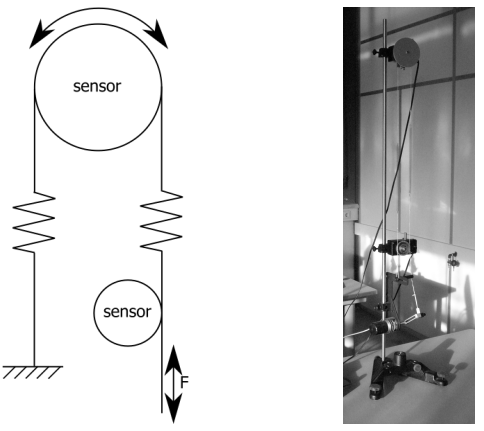
\includegraphics[width=1\textwidth]{oscillations/images/setup}
    \caption{The experimental setup}
    \label{fig:setup}
\end{figure}

During the first phase of the experiment the goal was to determine the natural frequency of the oscillator. To accomplish this first the magnet was removed and there was no driving force being supplied, instead the disc was manually rotated and its oscillations were recorded.
After these measurements the magnet was reïnstalled to introduce a damping term, the magnets position was adjusted so the oscillations would be damped after about 10 periods.

In the second phase a driving force was supplied by the electrical motor. First a couple of measurements of the amplitude of the oscillations and the frequency of the driving force were taken to gauge the voltage range that is to be used in finding the peak amplitude. After this two measurements were taken at seventeen different voltage levels, most of these measurements were conducted around the resonance frequency to get a more precise determination of the peak amplitude.

